\chapter{Standard Model and Quark Gluon Plasma}
\label{chap:Intro}
%% Note that the citations in this chapter use the journal and 
%% arXiv keys: I used the SLAC-SPIRES online BibTeX retriever 
%% to build my bibliography. There are also quite a few non-standard
%% macros, which come from my personal collection. You can have them
%% if you want, or I might get round to properly releasing them at 
%% some point myself.

%\chapterquote{Laws were made to be broken.}%
%{Christopher North, 1785-1854}%: Blackwood's Magazine May 1830

%Quark Gluon Plasma.\\
%Standard Model.\\
%Higgs Boson.\\
%Color Screening.\\
%Botomonia family \\
%$\Upsilon$ family \\

\section{Standard model and Quantun Chromodynamics}
%The central goal of relativistic heavy ion physics is the discovery of the new state of 
%strongly interacting matter that is called the quark-gluon plasma and the study of its properties. 
%In order to accomplish this goal, we need reliable signals for the formation of such a state.
\subsection{Standard model}
The Standard Model (SM) of particle physics is a theory of particle properties and
particle interactions \cite{SM}. It describes the strong, weak, and electromagnetic forces between
the fundamental particles of matter. Special relativity and quantum mechanics
form the basis for quantum field theory and the Standard Model.
The SM includes 12 elementary particles of spin $\frac{1}{2}$ known as fermions. The
fermions of the SM are classified according to how they interact (or equivalently,
by what charges they carry). There are six quarks (up, down, charm, strange, top,
bottom), and six leptons (electron, electron neutrino, muon, muon neutrino, tau, tau
neutrino) their properties are summarized in Table \ref{tab:StandardModelQuarksAndLeptons}. 
The quarks and leptons are grouped in three generations. 
The first generation contains the most stable particles which make most of the observed matter in the
universe, while the second and the third generations contain particles which decay to the lower
generation of particles.
The interactions among quarks and leptons occur via exchange of another type of particles
named bosons, see Table \ref{tab:StandardModelBoson}. The quarks and leptons have spin-1/2 while bosons are spin-1
particles. There are four fundamental interactions: strong, weak, electromagnetic and gravitational.
Each of the interactions has different strength and range of influence. Leptons
participate in gravitational, electromagnetic and weak interactions. Quarks on the other hand
can participate in all four interactions.
A graphical repersentation of all standard model particles can be seen in Figure \ref{fig:SM}.
The theory which describes the strong interaction between quarks and gluons is Quantum
Chromodynamics (QCD) and it will be described in the following sections


\begin{table}[bht]
\caption[]{Quarks and leptons properties. Every particle in the table has a corresponding
antiparticle with opposite charge. According to the Standard Model, the neutrino masses are
equal to zero. Observed neutrino oscillation suggests that the neutrinos have mass and their
experimental values are reported in the table}
\label{tab:StandardModelQuarksAndLeptons}
\begin{tabular}{lllll} 
Generation  &Name                                   &Symbol     &Electric charge        &Mass[MeV/c$^{2}$] \\
\hline
I           &Electron                              &e$^{-}$      &-1                     &0.511 \\
            &Electron neutrino                     &$\nu_{e}$    &0                      &$\leq$0.000225 \\ 

\hline
II         &Muon                                  &$\mu^{-}$      &-1                     &105.658 \\
            &Muon neutrino                         &$\nu_{\mu}$    &0                      &$\leq$ 0.19 \\ 

\hline
III         &Tau                                   &$\tau^{-}$     &-1                     &1776.82 \\
            &Tau neutrino                          &$\nu_{\tau}$    &0                      &$\leq$ 18.2 \\ 

\hline
             &                                    &Quarks         &                       &              \\

\hline
I            &Up                                   &u            &+$\frac{2}{3}$         &1.8$-$3.0 \\
             &Down                                 &d            &-$\frac{1}{3}$         &4.5$-$5.5 \\
\hline
II           &Charm                                &c            &+$\frac{2}{3}$         &1250$-$1300 \\
             &Strange                              &s            &-$\frac{1}{3}$         &90$-$100    \\

\hline
III          &Top                                &t            &+$\frac{2}{3}$         &172100$-$174900 \\
             &Bottom                             &b            &-$\frac{1}{3}$         &4150$-$4210    \\
\end{tabular}
\end{table} 


%\begin{figure}
%  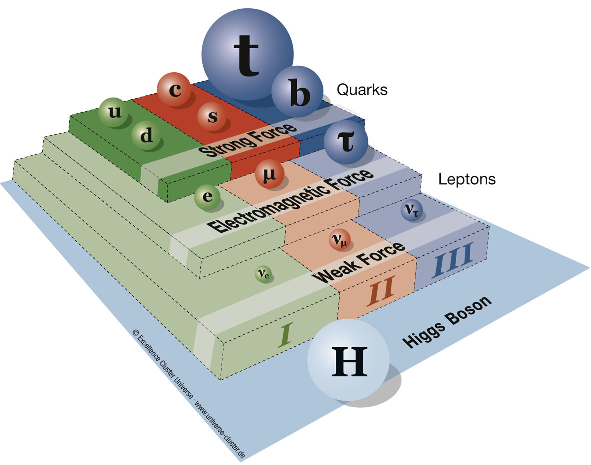
\includegraphics[width=\hugefigwidth]{chap_SMAndQGP_figures/StandardModel}
%  \caption[Standard Model]%
%  {Standard Model Figure}
%  \label{fig:SM}
%\end{figure}


%\begin{figure}
%  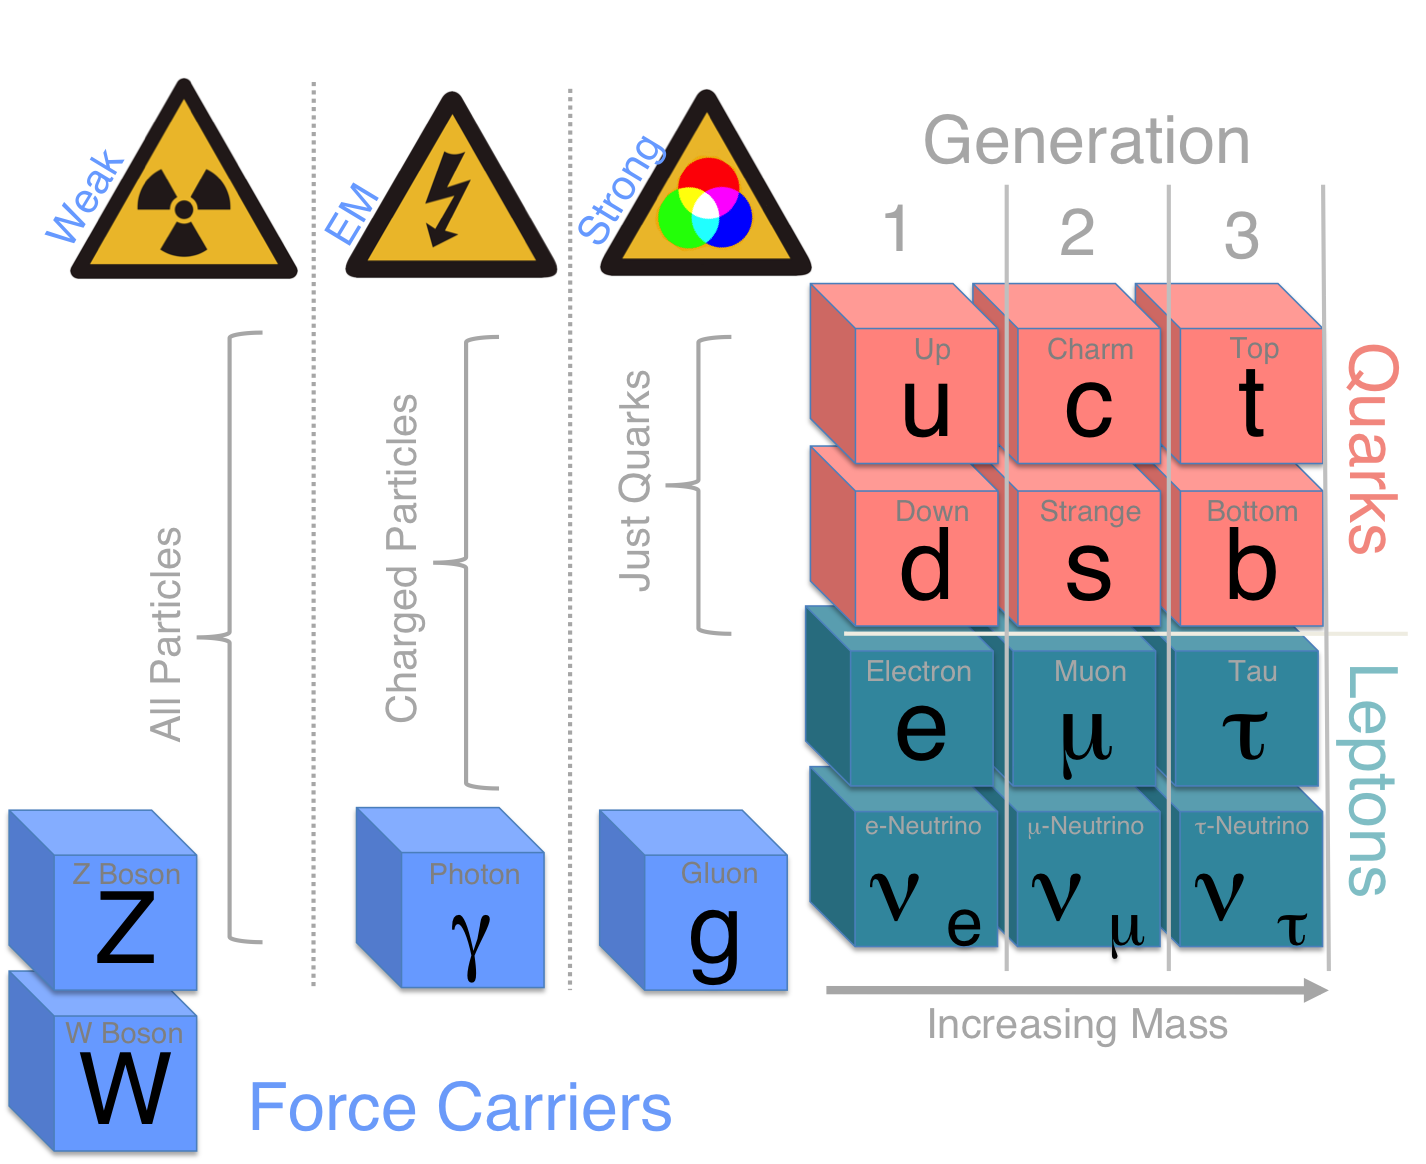
\includegraphics[width=\hugefigwidth]{chap_SMAndQGP_figures/SM_Fig4}
%  \caption[Standard Model 2]%
%  {Standard Model Figure 2}
%  \label{fig:SM2}
%\end{figure}



\begin{figure}
  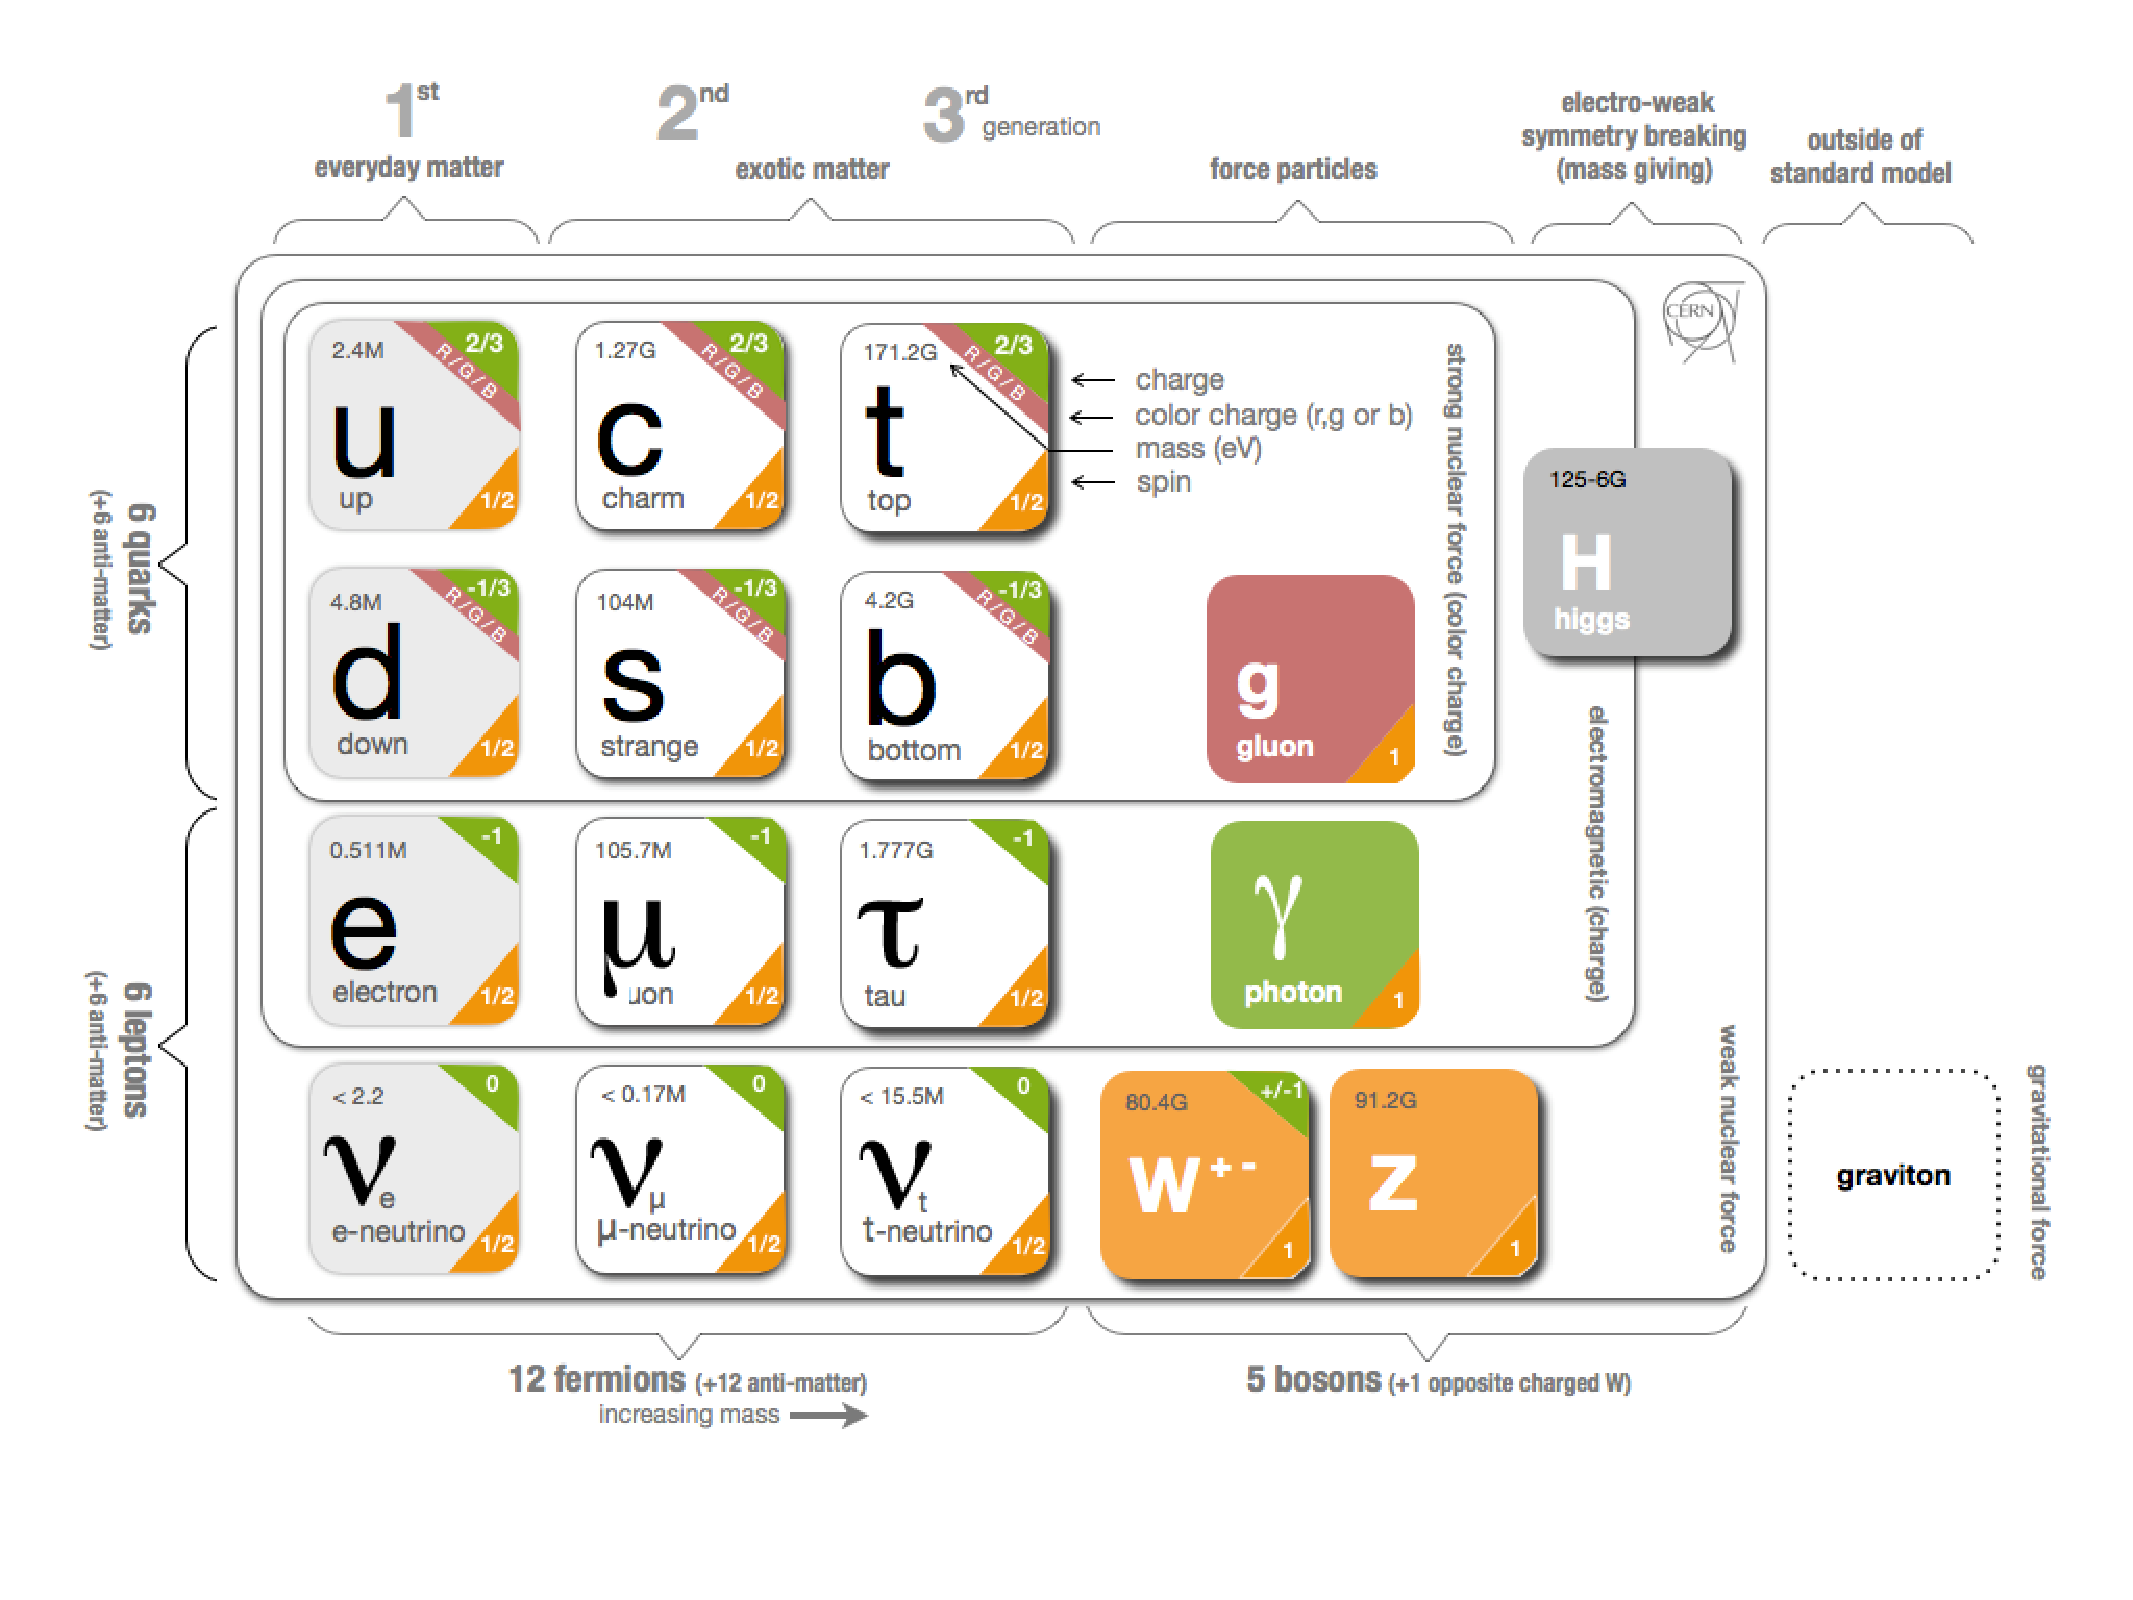
\includegraphics[width=\hugefigwidth]{chap_SMAndQGP_figures/Standard_model_infographic}
  \caption[Standard Model leptons and bosons]%
  {Standard Model leptons and bosons.}
  \label{fig:SM}
\end{figure}




\begin{table}[bht]
\caption[]{Boson properties}
\label{tab:StandardModelBoson}
\begin{tabular}{llll}
Name                                  &Force           &Electirc Charge         &Mass [GeV/c$^2$] \\
Symbol                                &Range(m)        &Color charge            &Strength        \\

\hline
Photon                                &Electromagnetic   &0                        &0                        \\
$\gamma$                              &$\infty$          &0                        &$\alpha$=$\frac{1}{137}$  \\

\hline
Gluon                                 &Strong            &0                        &0                        \\
g                                     &$10^{-15}$          &8 colored gluons         &$\alpha_s\,~$1, at high energy $\alpha_s \rightarrow$ 0\\

\hline
Z Boson                               &Weak               &0                        &91.187                        \\
Z$^0$                                 &$10^{-18}$           &0                        &$\alpha_z\,=\,10^{-6}$         \\

\hline
W Boson                              &Weak                &$\pm$1                   &80.399                        \\
W$^{\pm}$                             &$10^{-18}$            &0                        &$\alpha_W\,=\,10^{-6}$         \\
\end{tabular}
\end{table}




\subsection{Quantum Chromodynamics}

Quantum chromodynamics (QCD) \cite{QCD1,QCD2,QCD3,QCD4} is the field theory describing the
strong interactions of colored quarks and gluons. Color charge comes in three versions
(red, green and blue) that form a fundamental representation of the SU(3) group,
and is carried by both the quarks and gluons. Analogous to electric charge in quantum
electrodynamics (QED) \cite{QED1,QED2}, color charge is conserved in QCD, but since the gluons
carry color charge, they can interact with other gluons. This is not possible in QED,
as photons do not carry electric charge. The existence of self-coupling in QCD has
important implications for the scale dependence of the strong coupling.
In quantum field theory, the coupling constant describing the interaction between
two particles is an effective constant, which is dependent on the energy$-$scale Q$^2$ of
the interaction. In QED this dependence is only a weak one; in QCD, however, it
is very strong. The reason is the self-coupling of the gluons. The dependence of the
strong coupling constant $\alpha_s(Q^2)$ on Q$^2$ is known as a running coupling constant. In
perturbative QCD (pQCD), a first-order approximation yields:

\begin{equation}
\label{eq:QCD}
\alpha_s(Q^2) = \frac{1}{\beta_0\,ln(\frac{Q^2}{\Lambda^{2}_{QCD}})},\,\mbox{where}\,\beta_0 = \frac{33-n_f}{12\pi}
\end{equation}

Here, n$_f$ denotes the number of quark types with mass below Q$^2$, and $\Lambda_{QCD}$ represents
the characteristic scale of confinement. $\Lambda_{QCD}$ is determined by comparing predictions
with experimental data and is found to be on the order of 250 MeV \cite{QCD5}.


\begin{figure}
  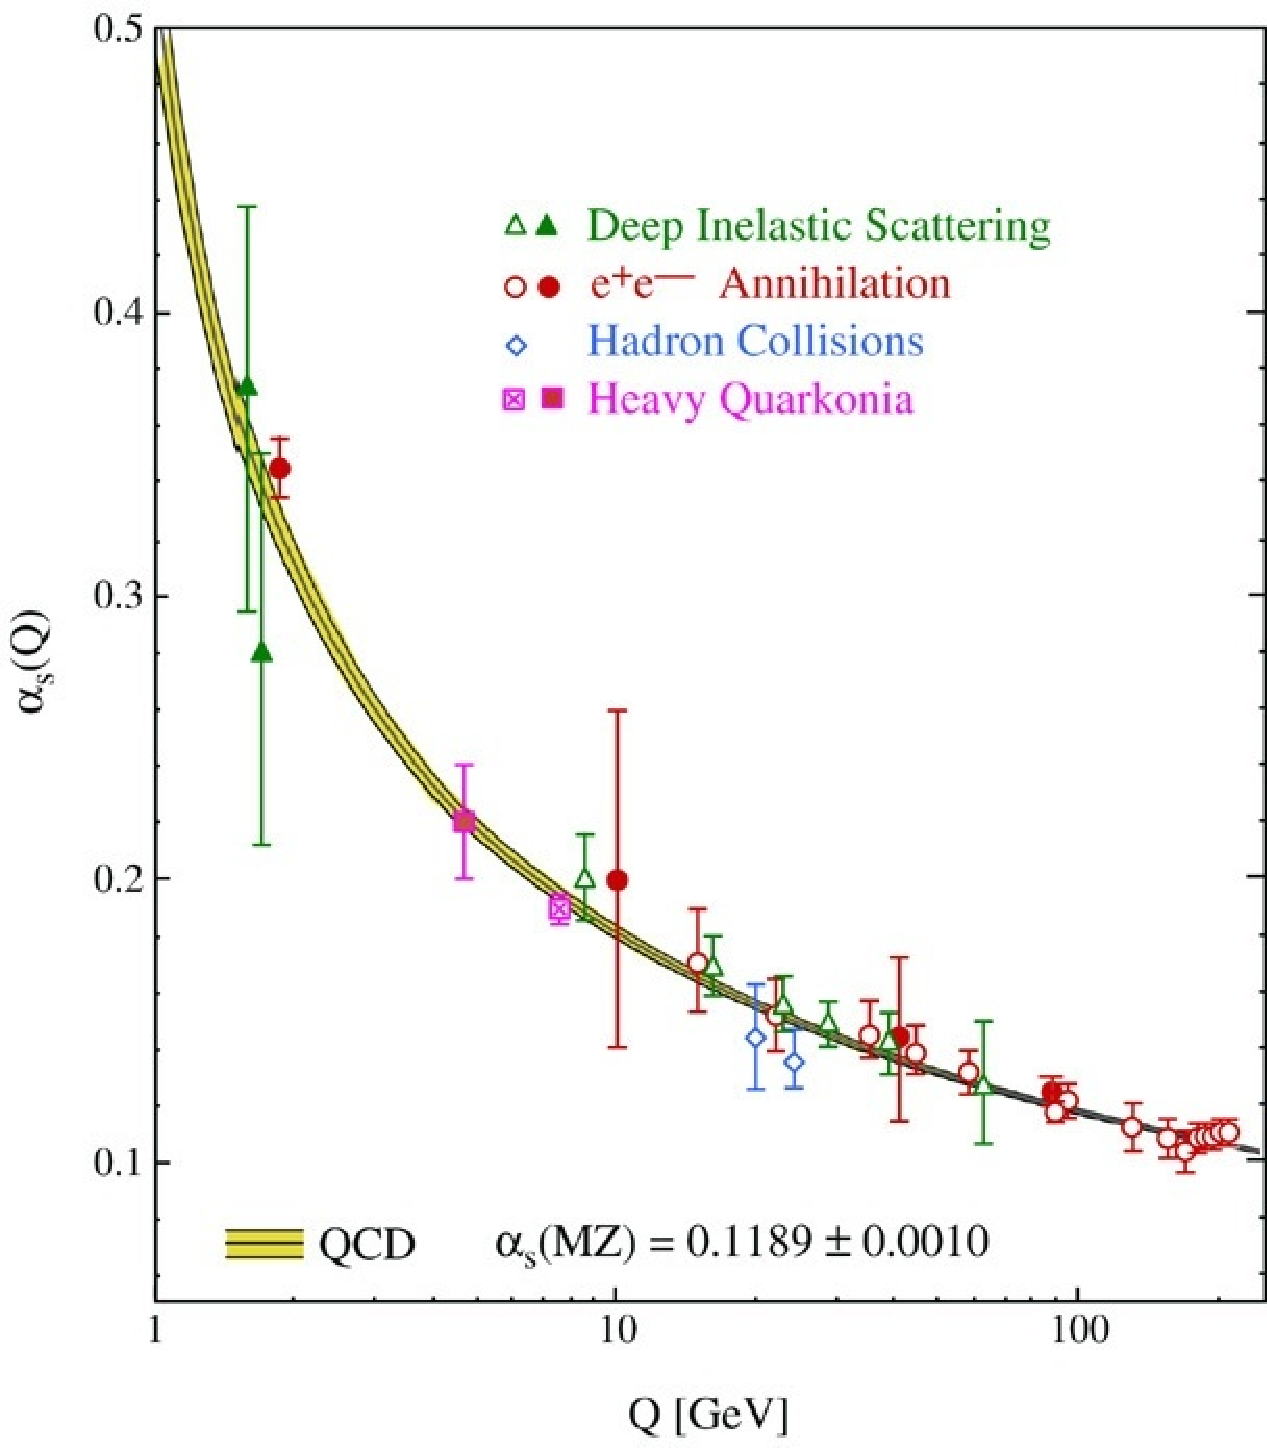
\includegraphics[width=\largefigwidth]{chap_SMAndQGP_figures/QCDAlpha_Prog}
  \caption[]{Figure shows a compilation of the values for $\alpha_s$, derived from many different experiments, and for different momenta Q of 
    the exchanged gluons. Gluon momentum is measured in GeV/c, and a logarithmic scale has been used to allow to show a bigger range of 
    values.}
  \label{fig:QCDAlpha}
\end{figure}



The Q$^2-$ dependence of the coupling strength corresponds to a dependence on quark
separation. For very small distances and corresponding high values of Q$^2$, the strong
coupling decreases, vanishing asymptotically as Q$^2\,\rightarrow\,\infty$ \ref{fig:QCDAlpha}. 
In the limit Q$^2\,\rightarrow\,\infty$, quarks
can be considered to be ``free''; this phenomenon is called asymptotic freedom. In
contrast, at large distances, the strong coupling increases substantially so that it is
not possible to detach individual quarks from hadrons. This phenomenon is called
confinement. In this regime, perturbation theory breaks down.
Quarks and gluons are not seen in experiments. Instead, they turn into hadrons,
which are observed in the detectors. This process is called hadronization. Hadronization
of quarks happens at a later time (t $\sim\,\frac{1}{\Lambda_{QCD}}$)
than the production process (t$\sim\,\frac{1}{Q}$). This is why the calculations 
of hadronic cross sections can be factorized into perturbative and non-perturbative parts.


\subsection{High Temperature QCD Matter}

The behavior of QCD at high temperatures or densities has long been of interest. In the first
few microseconds after the Big Bang, the universe would have had an enormous energy density, and
hence a very high temperature. It is expected that at such temperatures the component quarks
and gluons of normal hadronic matter have enough energy that they are no longer confined to their
usual bound states. This results in a phase transition between normal matter and a new state,
known as the Quark-Gluon Plasma (QGP) in analogy to electromagnetic plasmas in which the
electrons and ions are freed of their atomic bound states. A corresponding phase diagram can be
constructed, as shown in Figure \ref{fig:QCDPhaeDiagram}, which includes normal nuclear and hadronic matter, as well
as the QGP phase. In addition, other phases are expected to exist at higher net baryon chemical
potential, such as in neutron stars.


\begin{figure}
  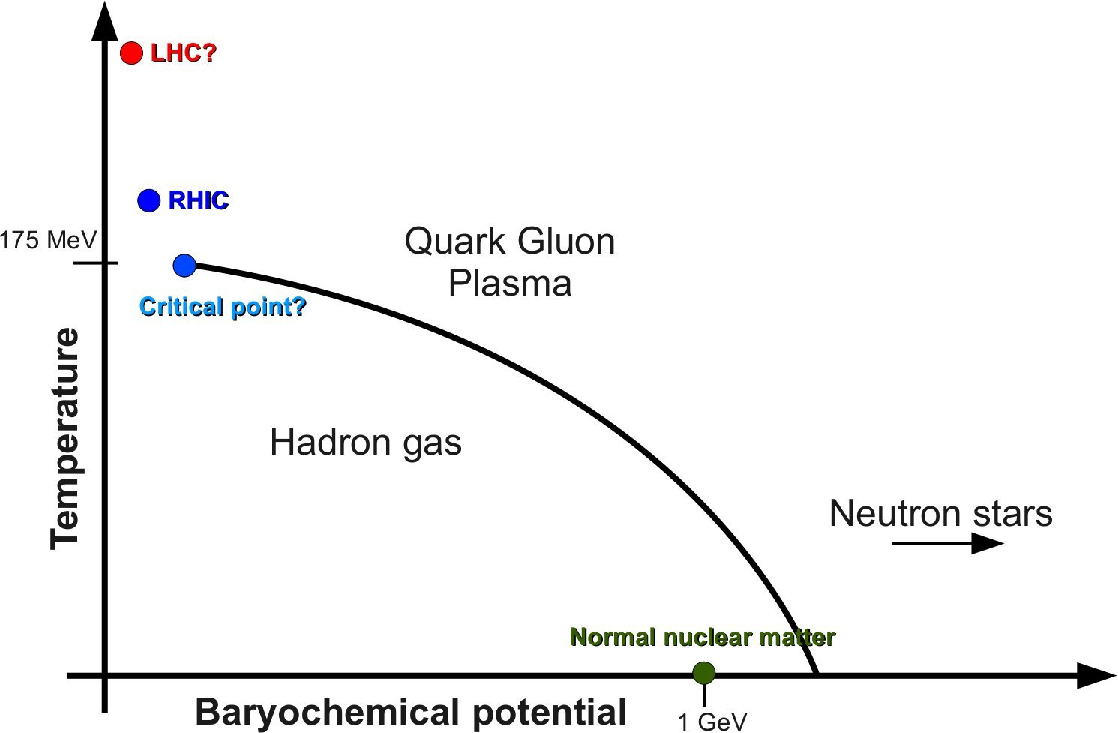
\includegraphics[width=\hugefigwidth]{chap_SMAndQGP_figures/QCDphasediagram1}
  \caption[QCD Phase diagram]
  {QCD phase diagram}
  \label{fig:QCDPhaeDiagram}
\end{figure}


\begin{figure}
  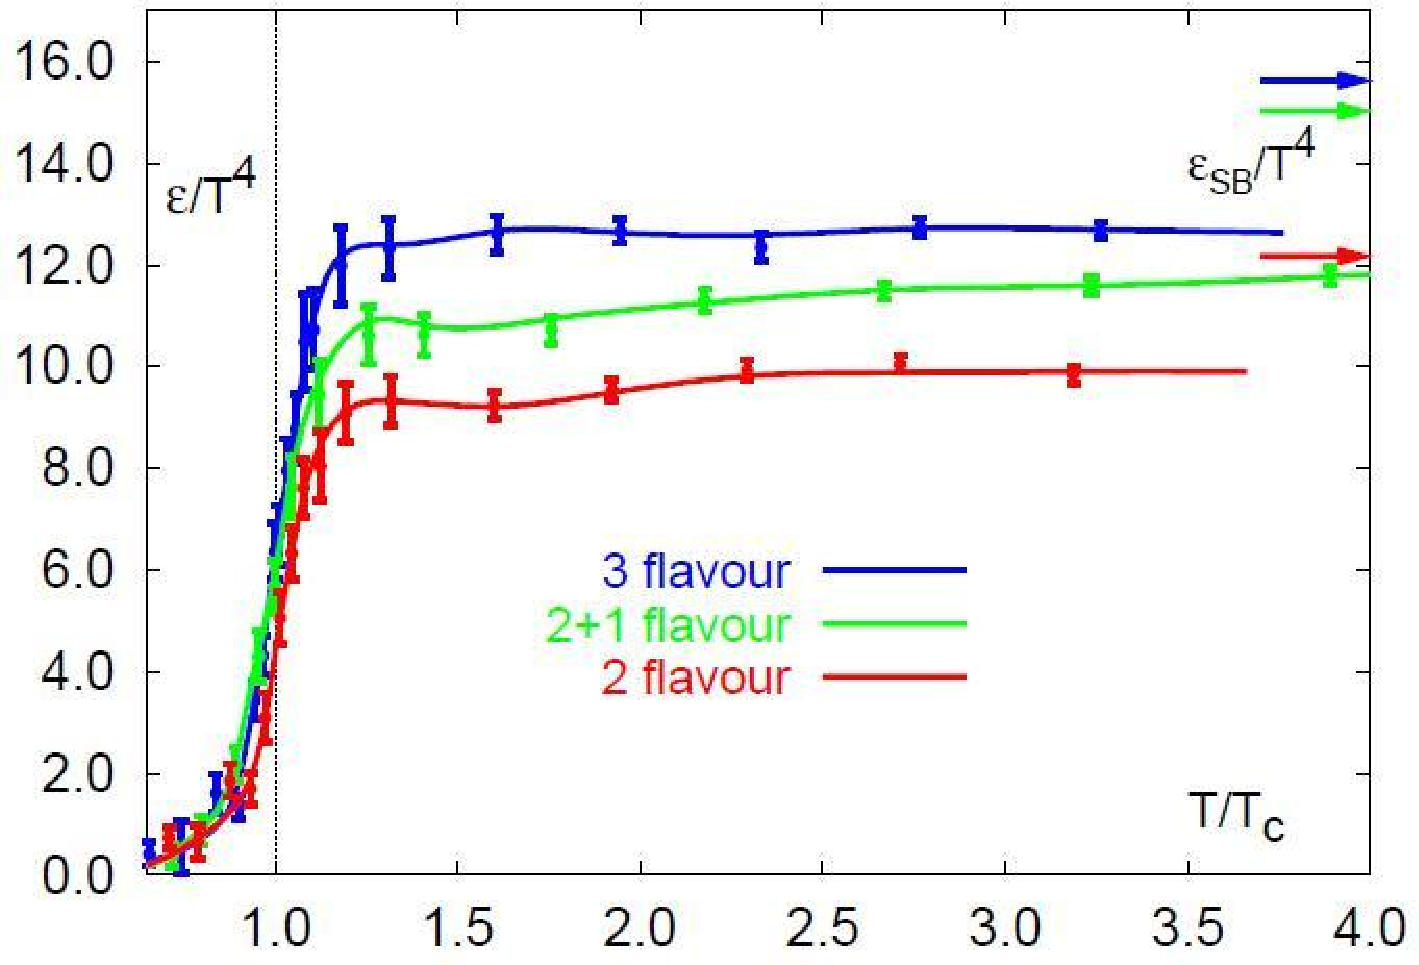
\includegraphics[width=\hugefigwidth]{chap_SMAndQGP_figures/LatticeQCD}
  \caption[QCD Phase diagram]
  {Energy density in units of T$^4$ as calculated in lattice QCD as calculated in \cite{LQCD1}. The
sharp rise at T$\sim$ T$_c$ corresponds to the phase transition to the QGP. On the right side the energy
density of a simple Stefan-Boltzmann gas of partons (as calculated in the text) is labeled.}
  \label{fig:LatticeQCD}
\end{figure}


Unfortunately, the QGP near the transition temperature is an inherently non-perturbative
regime, and other methods must be used to perform calculations. One way around this difficulty
is to perform numerical calculations using lattice QCD, which makes use of a Euclidean spacetime
grid to calculate the path integral of the QCD partition function. From there statistical and
thermodynamic properties such as temperature and free energy can be calculated.

Recently lattice QCD has been used to examine the phase transition to a QGP. It was found
that the transition temperature is Tc $\sim$ 170 MeV. This happens to lie very close to the Hagedorn
temperature T$_H\,\sim\,$ 160 MeV, the limiting temperature in high-energy hadronic collisions, above
which only the entropy of the thermodynamic system is increased (i.e. the number of hadronic
states produced) \cite{Hagedron}.

In order to create such a state of matter in the laboratory, heavy nuclei are collided at
relativistic velocities such that a portion of the large kinetic energy is converted to thermal energy.
The temperature dependence of the energy density can be naively calculated by assuming
the QGP is a Stefan-Boltzmann gas of massless, non-interacting particles \cite{WongBook,RamonaBook}. The partition
function for fermions $(-)$ and bosons $(+)$ is:


\begin{equation}
\label{eq:QCDPartFunc}
\mbox{ln Z(T,\mu,V)}=\frac{gV}{2\pi^2T}\int_{0}^{\infty}\frac{dk\,k^4}{3E}\, [ \frac{1}{e^{(E-\mu)/T}\pm1} + \frac{1}{e^{(E+\mu)/T}\pm1} ]
\end{equation}

If we assume that the number of quarks and anti-quarks are equal, then it can be shown that $\mu$=0.
For gluons (or other bosons), this becomes

\begin{eqnarray}
\label{eq:QCDPartFunc2}
\mbox{ln Z} &=  &g\frac{\pi^2}{90}VT^3 \,\,\mbox{(boson)}  \nonumber  \\
            &=  &g\frac{7\pi^2}{720}VT^3 \,\,\mbox{(fermions)} \nonumber \\
\end{eqnarray}

Now, since energy density is

 
\begin{eqnarray}
\label{eq:QCDEnDens}
\epsilon &= &(\frac{T^2}{V})( \frac{\delta \mbox{ln Z}}{\delta T}) \nonumber 
\end{eqnarray}

We can calculate

\begin{eqnarray}
\epsilon &= &(g_b + \frac{7}{8}g_f) \frac{\pi^2}{30} T^4 \\ 
\end{eqnarray}

where g$_{b,f}$ are the degeneracy numbers of the bosons,fermions as calculated below for gluons and
quarks+antiquarks:

\begin{eqnarray}
g_b &= &g_{gluon}             =(\mbox{(8 color states)(2 spin)}  \nonumber \\
g_f &= &g_{q}+g_{\overline{q}}   = \mbox{2(3 color)(2 spin)(n flavor)}    \nonumber \\
\end{eqnarray}

This gives us

\begin{eqnarray}
\epsilon &= &37\frac{\pi^2}{30}T^4 \mbox{(2 quark flavour)}\nonumber \\ 
         &= &47.5 \frac{\pi^2}{30}T^4 \mbox{(3 quark flavour)}\nonumber \\
\end{eqnarray}


for the energy density of a gas of massless partons.

Using lattice QCD it is possible to perform a more realistic calculation of the energy density.
Figure \ref{fig:LatticeQCD} shows such a calculation of the energy density \cite{LQCD1}. 
At sufficient temperature, this result shows the same T$^4$-scaling of the plasma energy density 
as calculated above. It should be noted that the calculation plateaus at $\sim$80$\%$ of the 
Stefan-Boltzmann gas of non-interacting partons. This
has sometimes been taken as evidence that the plasma weakly-interacting, but other calculations
have shown that even a strongly-interacting plasma could approach this limit \cite{LQCD2}.

As the medium expands and cools, it passes through several phases, as shown in Figure \ref{fig:HICollWhite}.
First hadronization will occur once the temperature becomes low enough that partons are confined
again. Next, kinetic freeze-out occurs when the expanding hadrons are too sparse to interact with
one another. At this point they will continue along their trajectories to be experimentally observed.
In order to extract any properties of the QGP medium, the evolution through other phases must
be accounted for as well. Hadronization in particular is not understood very well.

Topics of interest for the produced medium include the amount of thermalization of the
medium, how strongly-interacting the medium is, the nature of the phase transition itself, among
others.

Unfortunately, we are limited in our capabilities to experimentally study the properties of the
medium, due to its exceedingly short lifetime. Because of this we are constrained to probes that are
produced in the same collision as the medium, such as jets or heavy quarks from a hard scattering.


\begin{figure}
  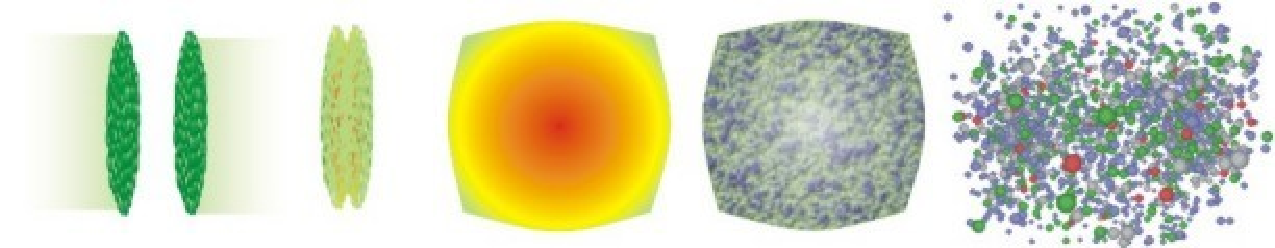
\includegraphics[width=\hugefigwidth]{chap_SMAndQGP_figures/HICollisions_White}
  \caption[HeavyIon Collisions]%
  {HI Collisions}
  \label{fig:HICollWhite}
\end{figure}

To understand the experimental measurements of these probes, however, we must understand their
initial production cross sections as well.


Our available probes and observables for studying the QGP medium include:
\begin{itemize}
 \item Elliptic flow of particles to study on the shear viscosity/entropy of the medium.
 \item Jet modification due to in-medium scattering and energy loss.
 \item Heavy quark flow as a measure of the medium thermalization.
 \item Hanbury-Brown-Twiss (HBT) interferometry to evaluate the distribution of matter.
 \item J/$\psi$ suppression above the QGP transition temperature as a signature of deconfinement.
 \end{itemize}

For a detailed review of experimental and theoretical status, see \cite{QGPThRev,QGPExpRev}.


To expand upon the last bullet item in the list, the QGP is expected to exhibit screening of the
interactions between color charges, similar to Debye screening of electric charges in electromagnetic
plasmas. Calculations of the screening length near the transition temperature have led to the
conclusion that the J/$\psi$  meson (a charm-anticharm bound state) is the right size to have its
constituent quarks Debye-screened from one another just above T$_c$. On the other hand  J/$\psi$ 
suppression is also affected by other effects like Cold Nucler Matter effect and recombination of
uncorelated charm-anticharm quark pair. It is observed that relative supperession $\Upsilon$ family
(bound state of b$\overline{b}$) can more roubest signature of Quark Gluon Plasma.  
 

%\begin{figure}
%  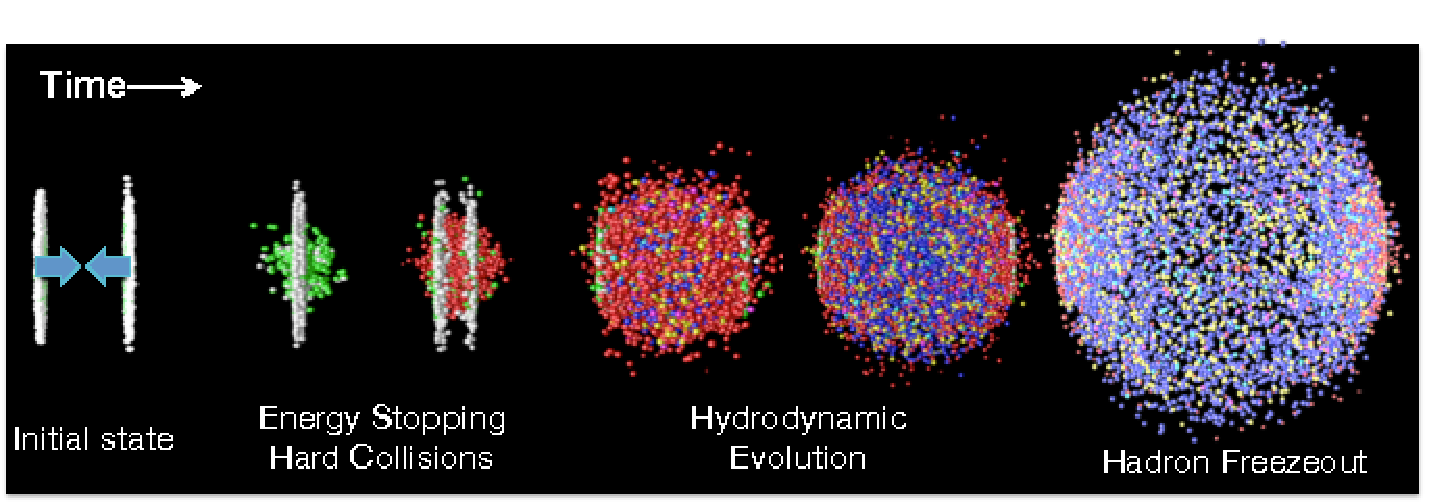
\includegraphics[width=\hugefigwidth]{chap_SMAndQGP_figures/black_heavy_ion_evolution}
%  \caption[HeavyIon Collisions time evolution]%
%  {HI Collisions time evolution}
%  \label{fig:HICollBlk}
%\end{figure}



%\begin{figure}
%  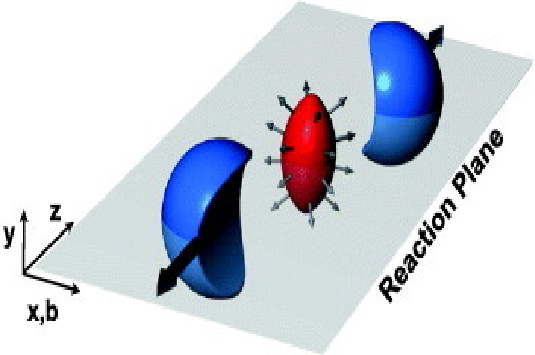
\includegraphics[width=\hugefigwidth]{chap_SMAndQGP_figures/ElipticFlow2}
%  \caption[Elitical flow in HI Collision]
%  {Elitical flow in HI Collision (v$_2$)}
%  \label{fig:V2}
%\end{figure}





